\documentclass[11pt,a4paper,oneside,notitlepage]{book}
\usepackage{amsmath}                    % Uitgebreide wiskundige mogelijkheden
\usepackage{amssymb}                    % Voor speciale symbolen zoals de verzameling Z, R...
\usepackage{makeidx}                    % Om een index te maken
\usepackage{url}						% Om url's te verwerken
\usepackage{fixltx2e}
\usepackage{textcomp}            
\usepackage{epstopdf}
%\usepackage{graphicx}                   % Om figuren te kunnen verwerken
\usepackage[pdftex]{graphicx}
%\usepackage[small,bf,hang]{caption2}    % Om de captions wat te verbeteren
\usepackage{xspace}                     % Magische spaties na een commando
\usepackage[latin1]{inputenc}           % Om niet ascii karakters rechtstreeks te
\usepackage{hyperref}
\usepackage{float}                      % Om nieuwe float environments aan te maken. Ook optie H!
%\usepackage{flafter}                   % Opdat floats niet zouden voorsteken
\usepackage{listings}                   % Voor het weergeven van letterlijke text en codelistings
\usepackage[round]{natbib}              % Voor auteur-jaar citaties.
\usepackage[nottoc]{tocbibind}			% Bibliografie en inhoudsopgave in ToC; zie tocbibind.dvi
\usepackage{marvosym}                   % Om het euro symbool te krijgen
%\usepackage{textcomp}                  % Voor onder andere graden celsius
%\usepackage{fancyhdr}                  % Voor fancy headers en footers.
%\usepackage[small,bf,hang]{caption2}	% Voor de captions te verbeteren
\usepackage[Gray,squaren,thinqspace,thinspace]{SIunits} % Elegant eenheden zetten 
\renewcommand{\baselinestretch}{1.35}   % De interlinie afstand wat vergroten.
%\usepackage[english,dutch]{babel}
\usepackage{flafter} %nieuw
\usepackage{lscape} %nieuw
\usepackage{fancyhdr}
\usepackage{graphicx}
\usepackage{amsmath, amssymb, amsbsy}
\usepackage{verbatim} 
\usepackage{float}
%\usepackage{subfigure}
\usepackage{subfig}
%\usepackage[small,bf,hang]{caption2}

% marges aanpassen
% (opmerking: moet *voor* inclusie van fancyhdr package komen)
\setlength{\hoffset}{-1in}
\setlength{\voffset}{-1in}
\setlength{\topmargin}{2cm}
\setlength{\headheight}{0.5cm}
\setlength{\headsep}{1cm}
\setlength{\oddsidemargin}{3.5cm}
\setlength{\evensidemargin}{3.5cm}
\setlength{\textwidth}{16cm}
\setlength{\textheight}{23.3cm}
\setlength{\footskip}{1.5cm}
\setlength{\parindent}{0cm}       
\setcounter{secnumdepth}{3} %nieuw


%Deftige fancy-header (hoofdstukken)
\pagestyle{fancy}
\fancyhf{}
\renewcommand{\headrulewidth}{0.5pt}
\fancyhf[HL]{\uppercase{\textit{\leftmark}}}
\fancyhf[HR]{\thepage}

\graphicspath{{images/}} % place of the figures

%\makeindex                              % Om een index te genereren.

\setcounter{MaxMatrixCols}{20}          % Max 20 kolommen in een matrix
\setcounter{tocdepth}{3}

% De headers die verschijnen bovenaan de bladzijden, herdefinieren:
\pagestyle{fancy}                       % Om aan te geven welke bladzijde stijl we gebruiken.
\fancyhf{}                              % Resetten van al de fancy settings.
\renewcommand{\headrulewidth}{0.4pt}      % Geen lijn onder de header. Zet dit op 0.4pt voor een mooie lijn.
\fancyhf[HL]{\nouppercase{\textit{\leftmark}}} % Links in de header zetten we de leftmark,
\fancyhead[HR]{\thepage}                % Rechts in de header het paginanummer.
% Activeer de volgende lijn en desactiveer de vorige om paginanummers onderaan gecentreerd te krijgen.
%\fancyhf[FC]{\thepage}                  % Paginanummers onderaan gecentreerd.

\newcommand{\cel}{$^{\circ}$C}


%%%%%%%%%%%%%%%%%%%%%%%%%
% Einde van de preamble.%
% Begin van de body:	  %
%%%%%%%%%%%%%%%%%%%%%%%%%

\begin{document}


\frontmatter

\title{iceLogo manual}
\author{Niklaas Colaert}
\author{Kenny Helsens}
\author{Lennart Martens}
\author{Jo�l Vandekerckhove}
\author{Kris Gevaert}


%  Titelblad

\begin{titlepage}

\fontsize{12pt}{14pt}\selectfont

\begin{center}

\begin{figure}[H] 
		\begin{center}
			
\includegraphics[width=3cm, height=4cm]{VIB.pdf}
			\hfill 
			
\includegraphics{ugent.pdf}
			
		\end{center}
\end{figure}



\vspace{0.3cm}


\vspace{0.8cm}
Department of Medical Protein Research, VIB, B-9000 Ghent, Belgium
\linebreak Department of Biochemistry, Ghent University, B-9000 Ghent, Belgium
\linebreak  \url{http://www.computationalproteomics.com}


\vspace{3.2cm}

	\begin{minipage}[c][4.5cm][c]{15cm}
	\begin{center}
	\fontsize{17.28pt}{21pt}\selectfont
	{\textsc{iceLogo manual}}
	\fontseries{m}
	\vspace{0.2cm}
	\fontsize{12pt}{14pt}\selectfont
	\linebreak Niklaas Colaert
	\linebreak Kenny Helsens
	\linebreak Jo�l Vandekerckhove
	\linebreak Kris Gevaert
	\linebreak Lennart Martens
	\end{center}
	\end{minipage}
	

\vspace{3.5cm}

\date{}
 \url{http://icelogo.ugent.be/}
\end{center}
\end{titlepage}



\tableofcontents

\mainmatter

\chapter*{Introduction}
Improved visualization of protein consensus sequences by iceLogo
\paragraph{}Large sequence-based datasets are often scanned for conserved sequence patterns to extract useful biological information (1). Sequence logos (2) were the first to visualize conserved patterns in oligonucleotide and protein sequences and rely on Shannon�s information theory to calculate the conservation level amongst all positions in a multiple sequence alignment. A sequence logo is a histogram-like presentation in which bars are vertical stacks of symbols, the stack height reflects the level of conservation and the height of individual symbols is a measure for their frequency at a given position. In a statistically sound manner however, no tool can compare an experimental peptide or protein sequence set to the background of species-specific natural occurrences of amino acids, to a position-specific background set, or to a background set that is influenced by the experimental protocol. In addition, underrepresented elements � non-tolerated amino acids or nucleotides � are generally not or not statistically well presented. 
\paragraph{}We recently introduce iceLogo (3) which takes the analysis and visualisation of consensus patterns in aligned peptide sequences to a new level. Instead of relying on information theory, iceLogo builds on probability theory. This theory takes the experimental set normally used to generate a sequence logo and compares it with a reference set. This reference set can be configurated by the user allowing it to be tailored to ideally approximate the expected background distribution. The experimental sequence set is generally a multiple sequence alignment of peptides that are expected to share sequence features. These two set will be used in a probability analysis and the result is shown in complementary illustrations like heat maps, amino acid parameter graphs and so-called iceLogos, which were all developed to aid analysis, visualisation and understanding of consensus sequences in an intuitive way.
\begin{itemize}
\item	1. Hulo, N. et al. Nucleic Acids Res 36, D245-249 (2008). 
\item	2. Schneider, T. D. & R. M. Stephens Nucleic Acids Res 18, 6097-6100 (1990). 
\item	3. Colaert, N. et al. Nature Methods 6, 786-787 (2009)
\end{itemize}



%chapter on the data visualization
\chapter{Different visualization methods}\label{description}


% ICELOGO
%%%%%%%
\section{iceLogo} \label{iceLogo}
\paragraph{}An iceLogo attemps to visualize a consensus sequence in a comprehensive manner just like sequence logos. However, it has two major benefits when compared to sequence logos. First, an iceLogo will always use a reference set. When no multiple sequence alignment can be given to create a reference set the option is to use the proteome background or sample a reference set from a protein FASTA file. Creation of the reference set is further described in sections \ref{web} and \ref{soap}. In this way, iceLogo always uses statistics to find over- and under-presented amino acids. Especially, the visualization of significantly under-represented amino acids is not present in sequence logos. Second, the dynamic nature of iceLogos, mainly the changing of the scoring system (see below), lets the user find changes in low abundant amino acids.
\paragraph{}On the iceLogo figure, significantly under- and over-represented amino acids will be visualized. For every position, the amino acid frequencies in the positive set will be compared with the frequencies in the reference set. An amino acid will be regulated if the Z-score is not a part of the confidence interval (this confidence interval is definied by the given p-value). The Z-score is calculated with the formula: Z-score = $\dfrac{X - \mu}{\sigma}$. The formula will calculate how many times the frequency (X) is deviated from the mean ($\mu$, the frequency of a specific amino acid on a specific position in the reference set) in terms of the standard deviation ($\sigma$). The way these standard deviations are calculated depends on the reference method used.
\paragraph{}Different scoring methods can be used in an iceLogo. The scoring method has an effect on the size of a regulated amino acid and the vertical position in the stack of regulated amino acids.

\begin{itemize}
\item \textbf{Fold change} When this method is selected the fold change will determine the size of the amino acid. In the following table the frequencies of two amino acids with their fold change are given. Although the percentage difference between the positive and the reference set is for both amino acid the same (6\%), the fold changes of the two amino acid show a large difference (7 $\Longleftrightarrow$ 2). The fold change scoring method let the user thus look for the regulation of low abundance amino acids.

\begin{center}
\begin{tabular}{c|c c}
Type & AA$_{1}$ & AA$_{2}$\\ 
\hline Frequency in experimental set (F+) & 7\%  & 12\% \\
Frequency in reference set (F-) & 1\% & 6\% \\ 
Percentage difference & 6\% & 6\% \\ 
Fold change $\dfrac{F+}{F-}$ & \textbf{\textit{7}} & \textbf{\textit{2}}\\ 
\end{tabular} 
\end{center}

If the calculated fold change (FC) is smaller than 1 the fold change will be converted via formula \ref{changeFC} to the converted fold change (FC$_{con}$). By this, the height of negatively regulated amino acid can be compared with the height of positively regulated amino acids. 
\begin{equation}
FC_{con} = \dfrac{1}{FC} * -1
\label{changeFC} 
\end{equation}
The following table gives an example of a converted fold change.
\begin{center}
\begin{tabular}{c|cc}
 & AA$_{1}$ & AA$_{2}$ \\
\hline Frequency experimental set (F+) & 12\% & 6\% \\
Frequencey reference set (F-) & 6\% & 12\% \\
Fold change (FC = $\dfrac{F+}{F-}$) & 2 & 0.5 \\
Converted fold change (FC$_{con}$) & 2 & \textbf{-2} \\
\end{tabular} 
\end{center}


\item \textbf{Percentage difference} This simple scoring method used the difference in frequency for an amino acid in the experimental set and the reference set as a measure of the height of a letter in the amino acid stack. This is the default scoring method.

\end{itemize}

\paragraph{}The color of the amino acids can dynamicly be changed when using the web application but cannot be changed when the iceLogo SOAP server is used. The amino acids will be colored pink if the amino acid is significantly regulated, and if this specific amino acid does not occure in the positive or reference set. If the scoring method is set to \textit{fold change}, the calculated height of a pink amino acid is infinite. Therefore, the height will be set to a specific value. Different scenarios exist for calculating this height.
\begin{itemize}
\item[] If only \textbf{one} amino acid is regulated and the calculated amino acid size is \textbf{infinite}, the height of the amino acid will be the same as the maximal height that can be visualized in the iceLogo.
\item[] If \textbf{more} amino acids are regulated and \textbf{all} the calculated amino acid sizes are \textbf{infinite}, the height of the amino acids will be the same as the maximal height that can be visualized in the iceLogo divided by the nummer of regultated amino acids on that position. All the regulated and infinite amino acids must be either over- or under-represented.
\item[] If \textbf{more} amino acids are regulated but \textbf{not all} the calculated amino acid sizes are \textbf{infinite}, the height of the infinite amino acids will 10 \% larger than the largest not infinite amino acid.
\end{itemize}


%HEAT MAP
%%%%%%%
\section{Heat map}
\paragraph{}A heat map attempts to visualize all the amino acid occurrences for all positions in one picture. The heat map is a 2D data matrix where every row is an amino acid and every column a position. At the right side of the heat map the gradient shows which p-values correlates with which colour. The Z-score is used for the calculation of the position and amino acid specific p-value and is calculated with the formula: Z-score = $\dfrac{X - \mu}{\sigma}$. The formula will calculate how many times the frequency (X) of that amino acid on that position is deviated from the mean ($\mu$, the frequency of a specific amino acid on a specific position in the reference set) in terms of the calculated standard deviation ($\sigma$). An error function (see formula \ref{erf}) can calculate a p-value for this Z-score.

\begin{equation}\label{erf}
P-value = erf(\dfrac{Z-score}{\sqrt{2}})
\end{equation}

\paragraph{}One cell in the heat map matrix will be coloured according to the calculated p-value for that position and amino acid. Only significantly up- and down-regulated elements - according to the given p-value - are coloured in respectively a shade of green and red. The non-regulated elements are coloured black.


\begin{figure}[H]
	\begin{center}
	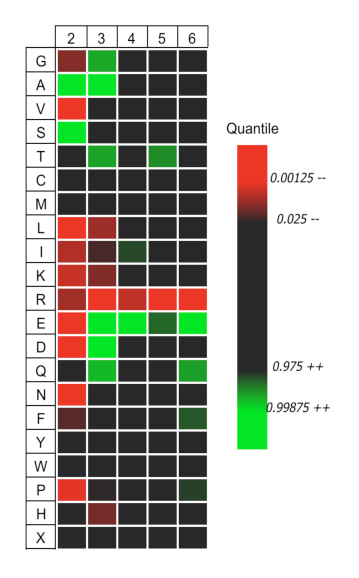
\includegraphics{heatmap.pdf}
	\caption{The figure shows the heatmap result of an iceLogo analysis. Increased or decreased amino acid frequencies are shown in a gradient of respectively green or red shades.}
	\label{fig:heatmap}
	\end{center}
\end{figure}


%SEQUENCE LOGO
%%%%%%%%%%%
\section{Sequence logo} \label{sequence logo}
\paragraph{}Sequence logos were originally created by Schneider and Stephens in 1990 and are used to visualize consensus sequences. Sequence logos are based on the \textit{information theory}. This theory states that a \textit{bit} is the amount of information necessary to choose between two equally probable choices. In a sequence logo the height of a stack of amino acids is thus calculated and presented in \textit{bits}. The height of one amino acid in such a stack reflects its frequency. 
\paragraph{}The maximal height of the stack is calculate with formula \ref{maxbits}. Where \textit{choices} stands for the number of possibile items. For DNA and RNA this is 4 and thus resulting in a maxBits value of 2. For proteins, there are 20 choices (amino acids) and the resulting maxBits is 4.32.
\begin{equation}
maxBits = \log_{2} choices
\label{maxbits} 
\end{equation}
\paragraph{}The final sequence logo height (sH) is calculated with formula \ref{sH}. In formula \ref{sH} the maxBits is substracted with the calBits. This calBits is calculated with formula \ref{calBits}. P$_{i}$  stands for the frequency of amino acid \textit{i}.
\begin{equation}
maxBits - calBits =sH
\label{sH} 
\end{equation}

\begin{equation}
calBits = - \Sigma (P_{i} \log_{2} P_{i})
\label{calBits} 
\end{equation}
\paragraph{}As a simple example, a set of 50 Arg (R) and 50 Lys (K) were used to create a sequence logo. The frequency of these amino acids are in both cases 50\%. Formula \ref{calBits} is used to calculate the calBits resulting in  1 (see formula \ref{calBitsTryp}).
\begin{equation}
calBits = 1 = - [ 0.5 \log_{2}(0.5) + 0.5 \log_{2}(0.5)]
\label{calBitsTryp} 
\end{equation}
The final sequence logo height can be calculated using formula \ref{sH}; 4.32 - 1 = 3.32. The height of the sequence logo in figure \ref{slTryp}.A is indeed 3.32.
\paragraph{}The iceLogo program can use the reference set for a background correction in sequence logos. iceLogo will calculate the height of the stack in the reference set and will substract it of the height of the stack in the positive set. This corrected sequence logo is presented in figure \ref{slTryp}.B.

\begin{figure}[H]
\begin{center}
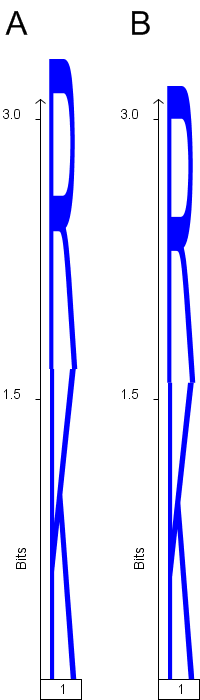
\includegraphics[scale=0.3]{slTryp.png}
\caption{These are both sequence logos generated with the iceLogo tool. Figure A is the normal sequence logo. Figure B is the reference set corrected sequence logo. Here the reference set is the human Swiss-Prot proteome.}
\label{slTryp}
\end{center}
\end{figure}

\paragraph{}10000 random human peptides were generated for the following example. The sequence logo without correction is given in figure \ref{10000random}.A. Figure \ref{10000random}.B gives the sequence logo with reference set correction. With this example, it's clearly shown that a background reduction in sequence logos has an important effect.

\begin{figure}[H]
\begin{center}
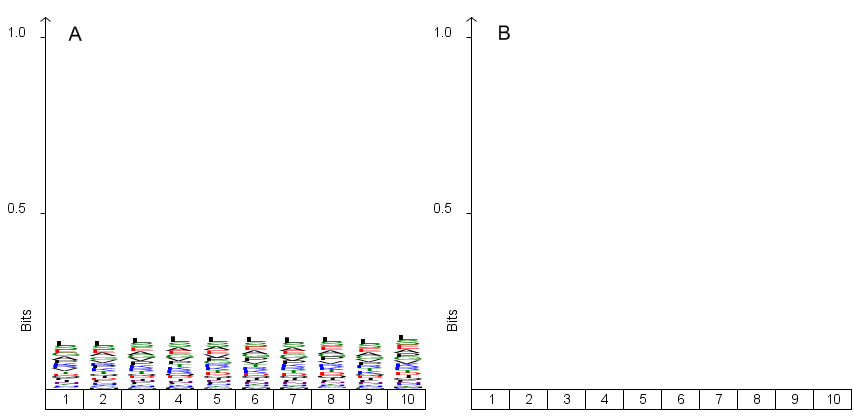
\includegraphics[scale=0.4]{10000random.png}
\caption{These are both sequence logos generated with the iceLogo tool. Figure A is the normal sequence logo. Figure B is the reference set corrected sequence logo. Both were created with 10000 random human peptides.}
\label{10000random}
\end{center}
\end{figure}

\paragraph{}The sequence logos generated by the web application and the iceLogo SOAP server are always created with a negative set correction.


% AA PARAMETER
%%%%%%%%%%
\section{Amino acid parameter graph}
\paragraph{} The iceLogo algorithm can visualize amino acid parameters. These parameters can be found in the AAindex1 database (\url{http://www.genome.jp/aaindex/}). The AAindex database is a database of numerical indices representing various published physicochemical and biochemical properties of amino acids. Currently, 544 indices are stored as matrices in this database and can be visualised by iceLogo. 
\paragraph{}The value for a specific position is calculated with formula \ref{aa} where P$_{i}$ is the frequency for amino acid \textit{i} and V$_{i}$ is the value for amino acid \textit{i} in the  amino acid parameter matrix used for the creation of the amino acid parameter graph. The values for different positions from the experimental set are linked by a green line. If two experimental sets are being analyzed, then this second set is linked by a blue line. Comparisons of two experimantal sets can only be done by the iceLogo SOAP server.
\begin{equation}
\Sigma P_{i} * V_{i}
\label{aa} 
\end{equation}

\paragraph{}The reference set is used to create a pink zone on the graph. This zone represents the non-regulated region. This non-regulated zone (the confidence interval) is determinded by the p-value and the background standard deviation. Two ways exist to create this background standard deviation.
\begin{enumerate}
\item When the static iceLogo method is used (available both in the web application and the iceLogo SOAP server) a standard deviation will be calculated for every position. This standard deviation will be calculated on 100 means. One such a mean, is the mean of the amino acid parameter values for N random (based on the reference set) amino acids and N is the sample size. This way, the reference set is used to simulate the background for an amino acid parameter.
\item When the sampling iceLogo method is used (only available via the iceLogo SOAP server), a background standard deviation will be calculated for every position. This standard deviation will be calculated on X parameter value means. X is the dimension of sampling. One such a mean, is the mean of the sampled amino acids parameter for a specific dimension. This way, the reference set is used as the background for an amino acid parameter. 
\end{enumerate} 
The red line in the pink zone represents the mean of the means used for the calculation of the background standard deviation.

% CORRELATION LINE
%%%%%%%%%%
\section{Correlation line}
\paragraph{} The iceLogo program can visualize the correlation between the different amino acids on one position. The correlation is calculated by using a substitution matrix. These substitution matrices can be found in the AAindex2 database (\url{http://www.genome.jp/aaindex/}). A substitution matrix holds values that describe the rate in which one amino acid changes in another amino acid over time. Currently, 94 substitution matrices are in this database and can be visualised by iceLogo. 
\paragraph{}For every amino acid in the set, the substitution score is calculated by tacking the mean of the substitution values of this amino acids with all the other amino acids in the set on that position. A substitution score is not normalized when the substitution score for one amino acid is multiplied by the substitution value of this amino acid with itself. If the set has 100 amino acids, 99 substution scores will be calculated for every amino acid. The mean of these 99 substitution score for the different positions from the experimental set are linked by a green line. If two experimental sets are being analyzed, then this second set is linked by a blue line.

\paragraph{}The reference set is used to create a gray zone on the graph. This zone represents the non-regulated region. This non-regulated zone (the confidence interval) is determinded by the p-value and the background standard deviation. Two ways exist to create this background standard deviation.
\begin{enumerate}
\item When the static iceLogo method is used (available both in the web application and the iceLogo SOAP server) a standard deviation will be calculated for every position. This standard deviation will be calculated on 100 means. One such a mean, is the mean of the amino acid parameter values for N random (based on the reference set) amino acids and N is the sample size. This way, the reference set is used to simulate the background for an amino acid parameter.
\item When the sampling iceLogo method is used (only available via the iceLogo SOAP server), a background standard deviation will be calculated for every position. This standard deviation will be calculated on X parameter value means. X is the dimension of sampling. One such a mean, is the mean of the sampled amino acids parameter for a specific dimension. This way, the reference set is used as the background for an amino acid parameter. 
\end{enumerate}
The dark line in the grey zone represents the mean of the means used for the calculation of the background standard 
deviation.

\section{Examples}
\subsection{iceLogo}
\paragraph{}An iceLogo was created for 452 human Granzyme B substrates (see \htmladdnormallink{Van Damme, P et al.}{http://www.ncbi.nlm.nih.gov/pubmed/18836177}). The processing sites of the subtrates of this protease are between positions 0 and 1. These sites were compared to a reference set. This reference set is the average amino acid occurrence for the human Swiss-Prot proteome.
\begin{figure}[H]
\begin{center}
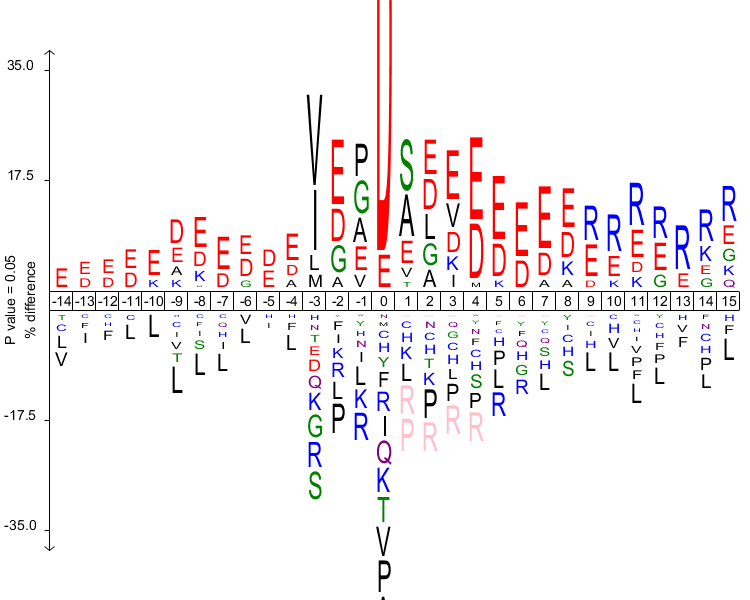
\includegraphics[scale=2]{example1.png}
\caption{Change this \htmladdnormallink{example}{http://icelogo.ugent.be/icelogoserver/logo.html?example=1}.}
\label{example1}
\end{center}
\end{figure}

\subsection{Heat map}
\paragraph{}A heat map was created for 452 human Granzyme B substrates (see \htmladdnormallink{Van Damme, P et al.}{http://www.ncbi.nlm.nih.gov/pubmed/18836177}). The processing sites of the subtrates of this protease are between positions 0 and 1.  These sites were compared to a reference set. This reference set is the average amino acid occurrence for the human Swiss-Prot proteome.
\begin{figure}[H]
\begin{center}
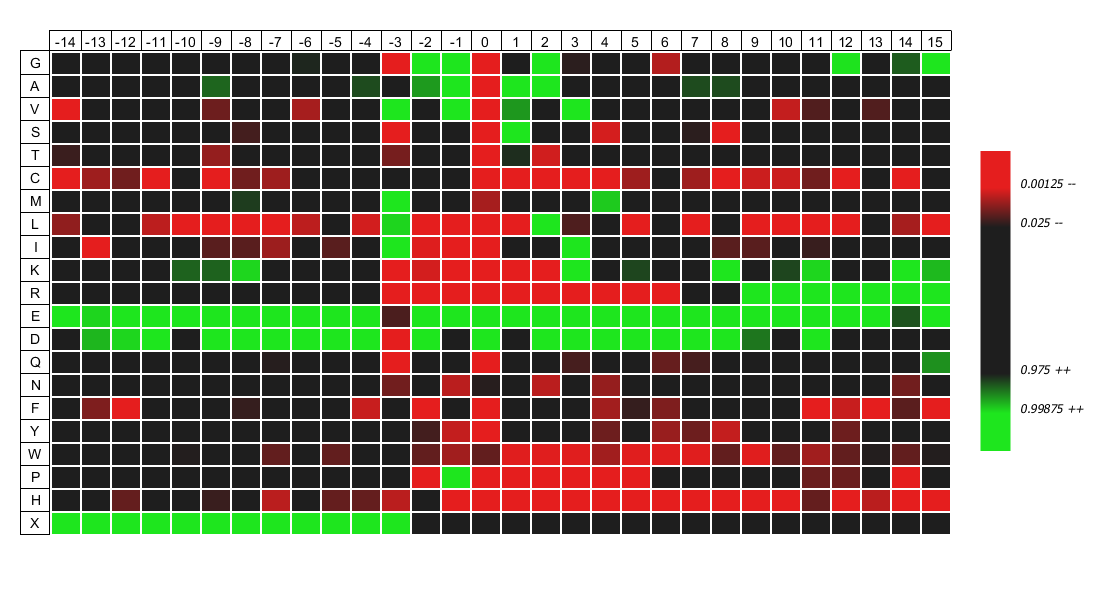
\includegraphics[scale=1.5]{example2.png}
\caption{Change this \htmladdnormallink{example}{http://icelogo.ugent.be/icelogoserver/logo.html?example=2}.}
\label{example2}
\end{center}
\end{figure}

\subsection{Sequence logo}
\paragraph{}A sequence logo was created for 452 human Granzyme B substrates (see \htmladdnormallink{Van Damme, P et al.}{http://www.ncbi.nlm.nih.gov/pubmed/18836177}). The processing sites of the subtrates of this protease are between positions 0 and 1.
\begin{figure}[H]
\begin{center}
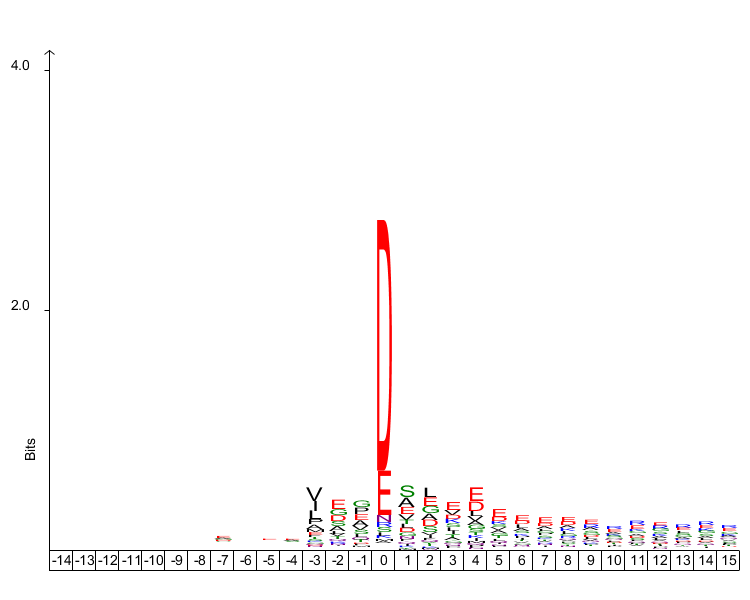
\includegraphics[scale=2]{example3.png}
\caption{Change this \htmladdnormallink{example}{http://icelogo.ugent.be/icelogoserver/logo.html?example=3}.}
\label{example3}
\end{center}
\end{figure}

\subsection{Filled logo}
\paragraph{}A filled logo was created for 452 human Granzyme B substrates (see \htmladdnormallink{Van Damme, P et al.}{http://www.ncbi.nlm.nih.gov/pubmed/18836177}). The processing sites of the subtrates of this protease are between positions 0 and 1.
\begin{figure}[H]
\begin{center}
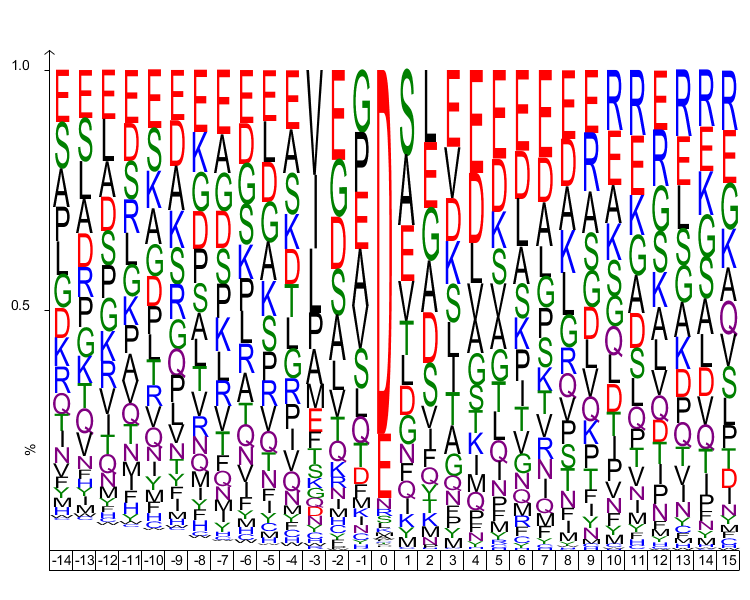
\includegraphics[scale=2]{example4.png}
\caption{Change this \htmladdnormallink{example}{http://icelogo.ugent.be/icelogoserver/logo.html?example=4}.}
\label{example4}
\end{center}
\end{figure}

\subsection{Amino acid parameter graph}
\paragraph{}An amino acid parameter graph was created for 452 human Granzyme B substrates (see \htmladdnormallink{Van Damme, P et al.}{http://www.ncbi.nlm.nih.gov/pubmed/18836177}). The processing sites of the subtrates of this protease are between positions 0 and 1. These sites were compared to a reference set. This reference set is the average amino acid occurrence for the human Swiss-Prot proteome. The amino acid parameter used was the "net charge".
\begin{figure}[H]
\begin{center}
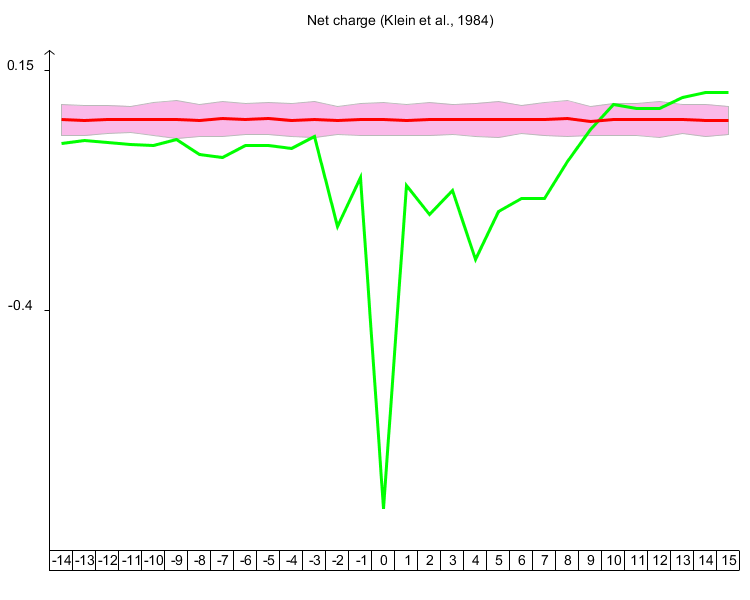
\includegraphics[scale=2]{example5.png}
\caption{Change this \htmladdnormallink{example}{http://icelogo.ugent.be/icelogoserver/logo.html?example=5}.}
\label{example5}
\end{center}
\end{figure}

\subsection{Correlation line}
\paragraph{}A correlation line was created for 52 mouse caspase 3 (see \htmladdnormallink{Demon, D et al.}{http://www.ncbi.nlm.nih.gov/pubmed/19759058}). The processing sites of the subtrates of this protease are between positions 0 and 1. These sites were compared to a reference set. This reference set is the average amino acid occurrence for the human Swiss-Prot proteome. The substitution matrix was set to "blosum 62".
\begin{figure}[H]
\begin{center}
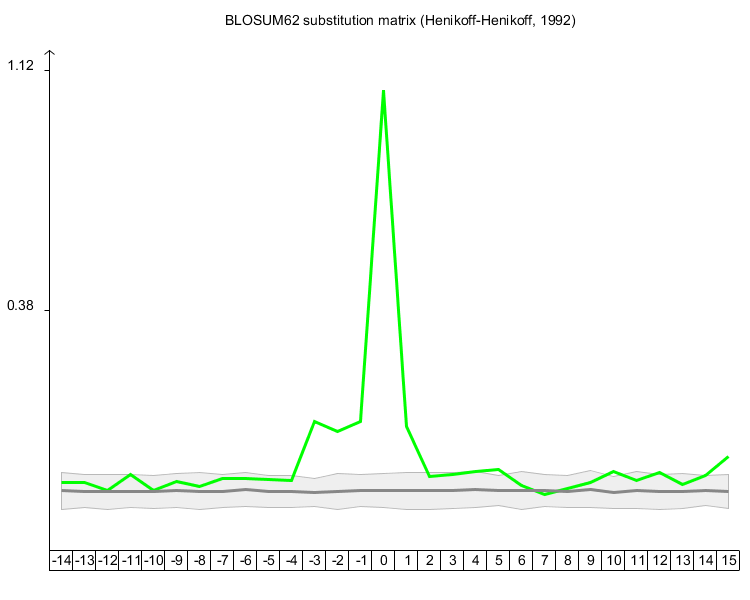
\includegraphics[scale=2]{example6.png}
\caption{Change this \htmladdnormallink{example}{http://icelogo.ugent.be/icelogoserver/logo.html?example=6}.}
\label{example6}
\end{center}
\end{figure}


\chapter{Statistics}
\paragraph{}The web application can only use the static reference method for the creation of iceLogo figures. The SOAP server on the other hand can use both the static and the sampling reference method.
\section{Static reference method}
\paragraph{}Two different types of reference set can be used in this method. One is the "fixed reference set" and the other is the "proteome background reference set". The first type of reference set is used in the different SOAP method that start with "getStaticReference...". In this type, a reference set will be created from a multiple sequence alignment. In the second reference method, the reference set will be created with the average occurrence of amino acids for a specific species in Swiss-Prot.
\paragraph{}Different parameters must be calculated before iceLogo can decide if the presence of a specific amino acid at a specific position is significant.
\begin{description}
\item[Sample size] The sample size is of great importance in the calculation of the standard deviation. The sample size is defined by the positive set and the reference set. When the sets are both multiple sequence alignments, the smallest set size (the multiple sequence alignment with the least sequence lines) will be used as the sample size. If the reference set is created with the proteome background method, the size of the positive set will be used as the sample size.
\item[Standard deviation] The standard deviation ($\sigma$) uses the sample size (N) and the frequency (f\%) of an amino acid in the the reference set and is calculated with formula \ref{sd}.
\end{description}

\begin{equation}
\sigma = \sqrt{\dfrac{f\%}{N}}
\label{sd} 
\end{equation}
\paragraph{}This calculated standard deviation will be used to calculate significances in the different visualization methods.


\section{Sampling reference set} \label{sampling}
\paragraph{}The second method is creating the reference set from a FASTA file. Sampling from a FASTA file comes both with advantages and drawbacks. When using static amino acid frequencies, one assumes that amino acid usage is generally equal to that of the whole proteome. But since this assumption is not actively tested by static methods, these methods might be prone to error. Therefore the major advantage of sampling from a FASTA sequence database is such that (unexpected) variation in amino acid usage is included in the sampling test. The major drawback is that the FASTA file must be repeatedly accessed and this computation comes with a time cost. Compared to instantaneously creating a static reference set, the sampling from the human subset of Swiss-Prot might last a minute or more. This is the reason why this type was not implemented in the web application and can only be accessed via the SOAP server.

\subsection{Statistics}
The reference set is the backbone for the statistics by reflecting the probability of finding an amino acid (AA) at random or under certain conditions. This is done as following. If the experimental set contains $n$ peptides, iceLogo samples $n$ peptides from a FASTA file and thereby calculates individual amino acid frequencies. If this process is iterated for at least 30 times, then the central limit theorem tells us we are allowed to infer normally distributed reference statistics with a mean and a standard deviation for each amino acid (\ref{eq_normal_dist_aa}). Finally the experimental sequence set, also containing n peptides, can then be tested against this reference distribution and conclusions can be drawn in terms of probability (\ref{eq_prob_aa}) by performing a $t$-test.

\begin{equation}\label{eq_normal_dist_aa}
N \left( \mu_{AA},\sigma_{AA} \right)
\end{equation}

\begin{equation}\label{eq_prob_aa}
P(AA) = \frac{1}{{\sigma_{AA} \sqrt {2\pi } }}e^{{{ - \left( {x - \mu_{AA} } \right)^2 } \mathord{\left/ {\vphantom {{ - \left( {x - \mu_{AA} } \right)^2 } {2\sigma_{AA} ^2 }}} \right. \kern-\nulldelimiterspace} {2\sigma_{AA} ^2 }}}
\end{equation}
      

\subsection{Sampling Types}\label{sampling_statistics}
\paragraph{}	iceLogo has various algorithms to sample peptides from the FASTA file. These are the so called sampling types which the user can choose and are listed below.
\paragraph{}	Among the distinct algorithms, the following variables are common:
\begin{description}
\item[sample size $n$] equals the number of peptides to calculate a single $Freq_{AA}$ per amino acid.
\item[iteration size $i$] equals the number of times the former calculation is iterated to estimate the mean $\bar{\mu}_{AA}$ and the standard deviation $\bar{\sigma}_{AA}$  on the frequency per amino acid.  
\end{description}
 
%Explains the random sampling.
\paragraph{Random}	The random sampling method calculates the probability to encounter an amino acid at random in the FASTA file. \\To do this, the algorithm reads $n$ protein sequences at random from the FASTA file. In each protein sequence, one amino acid is chosen at random and added to an amino acid counter. When $n$ amino acids have been added to this counter the $Freq_{AA}$ per amino acid is calculated. This process is then iterated $i$ times to estimate $\bar{\mu}_{Random_{AA}}$ and standard deviation $\bar{\sigma}_{Random_{AA}}$.
\paragraph{Terminal}\label{Terminal}	The terminal sampling method calculates the probability to encounter an amino acid at a given distance from a protein terminus in the FASTA file. \\To do this, the algorithm reads $n$ protein sequences at random from the FASTA file. In each protein sequence, a terminal peptide is retrieved (N-term or C-term) with length $l$ equal to the number of amino acids in an experimental peptide. The amino acids are added to $l$ separate amino acid counter for each position. When $n$ terminal peptides and their amino acids have been added to these counters, the $Freq_{AA_l}$ per amino acid is calculated for each position. This process is then iterated $i$ times to estimate $\bar{\mu}_{Terminal_{AA_l}}$ and standard deviation $\bar{\sigma}_{Terminal_{AA_l}}$.
\paragraph{Regional}	The regional sampling method calculates the probability to encounter an amino acid in the region around an anchored experimental position. \\To do this, the algorithm first analyses the amino acid frequency at an anchored position $Freq_{AA_anchor}$  in the experimental set. For example, a experimental sequence set with phosphorylated peptides anchored to the phosphorylation site has $Freq_{AA_{Ser}} =70\%$ and $Freq_{AA_{Thr}} =30\%$. Then the algorithm reads $n$ protein sequences at random from the FASTA file. In each protein sequence, a regional peptide around the anchor site is retrieved with length $l$ equal to the number of amino acids in an experimental peptide. In the example, $0.70\:x\:n$ regional peptides have a Ser anchor and $0.30\:x\:n$ regional peptides have a Thr anchor. The amino acids are then added to $l$ separate amino acid counter for each position around the anchor site. When $n$ regional peptides and their amino acids have been added to these counters, the $Freq_{AA_l}$ per amino acid is calculated for each position around the anchor. This process is then iterated $i$ times to estimate $\bar{\mu}_{Regional_{AA_l}}$ and standard deviation $\bar{\sigma}_{Regional_{AA_l}}$.

	
	These options enable extra fine-tuning of the sampling algorithm.
	\begin{description}
		
		\item[Terminal - Anchor start position] Set the offset to start terminal sampling 
		\item[Terminal - Direction] Set the direction to either sample peptides from the N- or C-terminal end of the protein. 
		\item[Regional - Sampling position] This value indicates which position the iceLogo algorithm has take as anchored experimental position.  
	\end{description}



%chapter on the creation of visualizations
\chapter{Creating different visualizations}\label{creation}
\section{Web application} \label{web}
\paragraph{}Creating a visualization is very easy with the web application. The experimental set must be given as a multiple sequence alignment. The exact format of the mutliple sequence alignment can be seen on the web page when the sample data is loaded (click "Load Human Granzyme B substrates as sample data" just beneath the experimental set text area). The reference set can also be a mutiple sequence alignment. This can be set in the "Reference set" text area. However, a Swiss-Prot composition for a specific species can also be selected. This is done by checking the "Swiss-Prot composition" checkbox and selecting a valid scientific species name in the text box next to the checkbox. 
\paragraph{}Generating the image is done by clicking the "Generate" button below the sequence set text areas. Whenever an image is created this can also be viewed in different image types. The default visualized image is a jpeg. A pdf, tiff, png and svg version of this image can be found when the links -that appear after the loading of the image below the "Generate" button is done- are clicked. If the user created more than one image in one session these can be revisualized by clicking the "next" and "previous" buttons below the "Generate" button.
\paragraph{}Additional image and iceLogo parameters can be set below the "Generate" button. This include choosing the scoring type, the visualization method, the colors of the letters, the size of the image ... . 


\section{SOAP server} \label{soap}
\paragraph{}A SOAP server can be accessed via \url{http://icelogo.ugent.be/icelogoserver/services/icelogo}. More information about this SOAP server can be found on \url{http://icelogo.ugent.be/icelogoserver/soap.html}. The wsdl file describing these services and methods can be found on \url{http://icelogo.ugent.be/icelogoserver/icelogo.wsdl}. 
\backmatter

\end{document}